% Created by tikzDevice version 0.10.1 on 2016-05-08 18:26:47
% !TEX encoding = UTF-8 Unicode
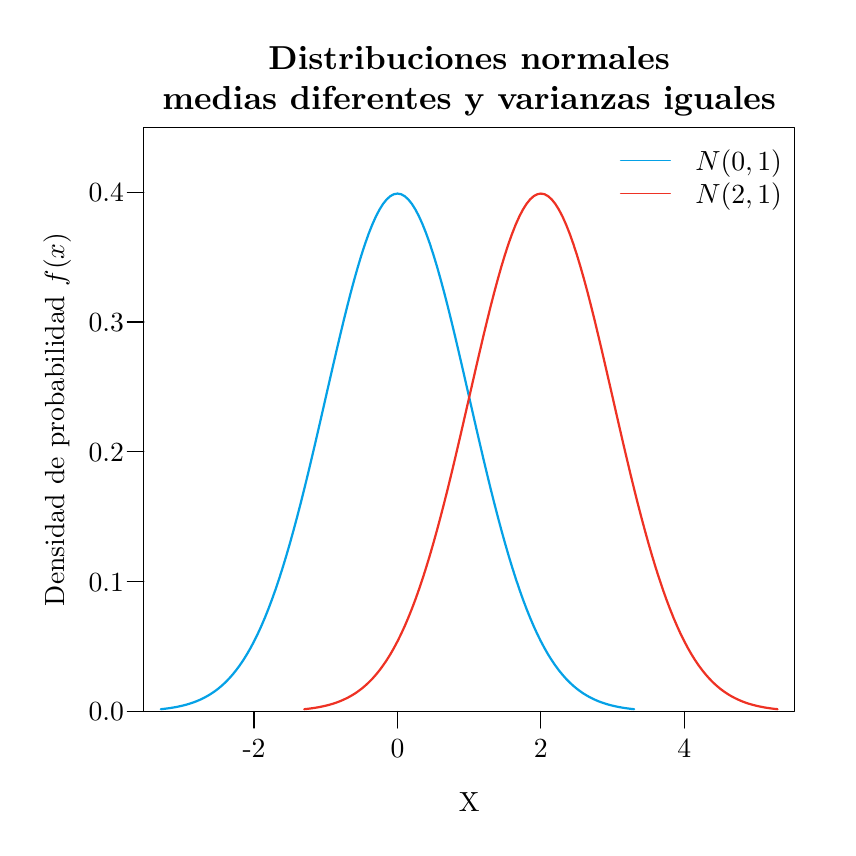
\begin{tikzpicture}[x=1pt,y=1pt]
\definecolor{fillColor}{RGB}{255,255,255}
\path[use as bounding box,fill=fillColor,fill opacity=0.00] (0,0) rectangle (289.08,289.08);
\begin{scope}
\path[clip] ( 42.00, 42.00) rectangle (277.08,253.08);
\definecolor{drawColor}{RGB}{5,161,230}

\path[draw=drawColor,line width= 0.8pt,line join=round,line cap=round] ( 48.12, 42.81) --
	( 49.41, 42.95) --
	( 50.71, 43.12) --
	( 52.00, 43.31) --
	( 53.30, 43.53) --
	( 54.59, 43.79) --
	( 55.89, 44.08) --
	( 57.18, 44.41) --
	( 58.48, 44.79) --
	( 59.78, 45.22) --
	( 61.07, 45.71) --
	( 62.37, 46.27) --
	( 63.66, 46.89) --
	( 64.96, 47.59) --
	( 66.25, 48.37) --
	( 67.55, 49.25) --
	( 68.85, 50.22) --
	( 70.14, 51.31) --
	( 71.44, 52.50) --
	( 72.73, 53.83) --
	( 74.03, 55.29) --
	( 75.32, 56.89) --
	( 76.62, 58.64) --
	( 77.92, 60.55) --
	( 79.21, 62.63) --
	( 80.51, 64.89) --
	( 81.80, 67.33) --
	( 83.10, 69.95) --
	( 84.39, 72.78) --
	( 85.69, 75.80) --
	( 86.98, 79.03) --
	( 88.28, 82.47) --
	( 89.58, 86.12) --
	( 90.87, 89.97) --
	( 92.17, 94.03) --
	( 93.46, 98.29) --
	( 94.76,102.75) --
	( 96.05,107.40) --
	( 97.35,112.23) --
	( 98.65,117.23) --
	( 99.94,122.38) --
	(101.24,127.67) --
	(102.53,133.09) --
	(103.83,138.60) --
	(105.12,144.19) --
	(106.42,149.83) --
	(107.71,155.50) --
	(109.01,161.17) --
	(110.31,166.81) --
	(111.60,172.39) --
	(112.90,177.88) --
	(114.19,183.25) --
	(115.49,188.47) --
	(116.78,193.50) --
	(118.08,198.30) --
	(119.38,202.86) --
	(120.67,207.14) --
	(121.97,211.11) --
	(123.26,214.74) --
	(124.56,218.01) --
	(125.85,220.90) --
	(127.15,223.37) --
	(128.44,225.43) --
	(129.74,227.04) --
	(131.04,228.20) --
	(132.33,228.90) --
	(133.63,229.13) --
	(134.92,228.90) --
	(136.22,228.20) --
	(137.51,227.04) --
	(138.81,225.43) --
	(140.11,223.37) --
	(141.40,220.90) --
	(142.70,218.01) --
	(143.99,214.74) --
	(145.29,211.11) --
	(146.58,207.14) --
	(147.88,202.86) --
	(149.17,198.30) --
	(150.47,193.50) --
	(151.77,188.47) --
	(153.06,183.25) --
	(154.36,177.88) --
	(155.65,172.39) --
	(156.95,166.81) --
	(158.24,161.17) --
	(159.54,155.50) --
	(160.84,149.83) --
	(162.13,144.19) --
	(163.43,138.60) --
	(164.72,133.09) --
	(166.02,127.67) --
	(167.31,122.38) --
	(168.61,117.23) --
	(169.91,112.23) --
	(171.20,107.40) --
	(172.50,102.75) --
	(173.79, 98.29) --
	(175.09, 94.03) --
	(176.38, 89.97) --
	(177.68, 86.12) --
	(178.97, 82.47) --
	(180.27, 79.03) --
	(181.57, 75.80) --
	(182.86, 72.78) --
	(184.16, 69.95) --
	(185.45, 67.33) --
	(186.75, 64.89) --
	(188.04, 62.63) --
	(189.34, 60.55) --
	(190.64, 58.64) --
	(191.93, 56.89) --
	(193.23, 55.29) --
	(194.52, 53.83) --
	(195.82, 52.50) --
	(197.11, 51.31) --
	(198.41, 50.22) --
	(199.70, 49.25) --
	(201.00, 48.37) --
	(202.30, 47.59) --
	(203.59, 46.89) --
	(204.89, 46.27) --
	(206.18, 45.71) --
	(207.48, 45.22) --
	(208.77, 44.79) --
	(210.07, 44.41) --
	(211.37, 44.08) --
	(212.66, 43.79) --
	(213.96, 43.53) --
	(215.25, 43.31) --
	(216.55, 43.12) --
	(217.84, 42.95) --
	(219.14, 42.81);
\end{scope}
\begin{scope}
\path[clip] (  0.00,  0.00) rectangle (289.08,289.08);
\definecolor{drawColor}{RGB}{0,0,0}

\path[draw=drawColor,line width= 0.4pt,line join=round,line cap=round] ( 81.80, 42.00) -- (237.28, 42.00);

\path[draw=drawColor,line width= 0.4pt,line join=round,line cap=round] ( 81.80, 42.00) -- ( 81.80, 36.00);

\path[draw=drawColor,line width= 0.4pt,line join=round,line cap=round] (133.63, 42.00) -- (133.63, 36.00);

\path[draw=drawColor,line width= 0.4pt,line join=round,line cap=round] (185.45, 42.00) -- (185.45, 36.00);

\path[draw=drawColor,line width= 0.4pt,line join=round,line cap=round] (237.28, 42.00) -- (237.28, 36.00);

\node[text=drawColor,anchor=base,inner sep=0pt, outer sep=0pt, scale=  1.00] at ( 81.80, 25.20) {-2};

\node[text=drawColor,anchor=base,inner sep=0pt, outer sep=0pt, scale=  1.00] at (133.63, 25.20) {0};

\node[text=drawColor,anchor=base,inner sep=0pt, outer sep=0pt, scale=  1.00] at (185.45, 25.20) {2};

\node[text=drawColor,anchor=base,inner sep=0pt, outer sep=0pt, scale=  1.00] at (237.28, 25.20) {4};

\path[draw=drawColor,line width= 0.4pt,line join=round,line cap=round] ( 42.00, 42.00) -- ( 42.00,229.63);

\path[draw=drawColor,line width= 0.4pt,line join=round,line cap=round] ( 42.00, 42.00) -- ( 36.00, 42.00);

\path[draw=drawColor,line width= 0.4pt,line join=round,line cap=round] ( 42.00, 88.91) -- ( 36.00, 88.91);

\path[draw=drawColor,line width= 0.4pt,line join=round,line cap=round] ( 42.00,135.81) -- ( 36.00,135.81);

\path[draw=drawColor,line width= 0.4pt,line join=round,line cap=round] ( 42.00,182.72) -- ( 36.00,182.72);

\path[draw=drawColor,line width= 0.4pt,line join=round,line cap=round] ( 42.00,229.63) -- ( 36.00,229.63);

\node[text=drawColor,anchor=base east,inner sep=0pt, outer sep=0pt, scale=  1.00] at ( 34.80, 38.56) {0.0};

\node[text=drawColor,anchor=base east,inner sep=0pt, outer sep=0pt, scale=  1.00] at ( 34.80, 85.46) {0.1};

\node[text=drawColor,anchor=base east,inner sep=0pt, outer sep=0pt, scale=  1.00] at ( 34.80,132.37) {0.2};

\node[text=drawColor,anchor=base east,inner sep=0pt, outer sep=0pt, scale=  1.00] at ( 34.80,179.28) {0.3};

\node[text=drawColor,anchor=base east,inner sep=0pt, outer sep=0pt, scale=  1.00] at ( 34.80,226.18) {0.4};

\path[draw=drawColor,line width= 0.4pt,line join=round,line cap=round] ( 42.00, 42.00) --
	(277.08, 42.00) --
	(277.08,253.08) --
	( 42.00,253.08) --
	( 42.00, 42.00);
\end{scope}
\begin{scope}
\path[clip] (  0.00,  0.00) rectangle (289.08,289.08);
\definecolor{drawColor}{RGB}{0,0,0}

\node[text=drawColor,anchor=base,inner sep=0pt, outer sep=0pt, scale=  1.20] at (159.54,274.09) {\bfseries Distribuciones normales};

\node[text=drawColor,anchor=base,inner sep=0pt, outer sep=0pt, scale=  1.20] at (159.54,259.69) {\bfseries medias diferentes y varianzas iguales};

\node[text=drawColor,anchor=base,inner sep=0pt, outer sep=0pt, scale=  1.00] at (159.54,  6.00) {X};

\node[text=drawColor,rotate= 90.00,anchor=base,inner sep=0pt, outer sep=0pt, scale=  1.00] at ( 13.20,147.54) {Densidad de probabilidad $f(x)$};
\end{scope}
\begin{scope}
\path[clip] ( 42.00, 42.00) rectangle (277.08,253.08);
\definecolor{drawColor}{RGB}{238,50,36}

\path[draw=drawColor,line width= 0.8pt,line join=round,line cap=round] ( 99.94, 42.81) --
	(101.24, 42.95) --
	(102.53, 43.12) --
	(103.83, 43.31) --
	(105.12, 43.53) --
	(106.42, 43.79) --
	(107.71, 44.08) --
	(109.01, 44.41) --
	(110.31, 44.79) --
	(111.60, 45.22) --
	(112.90, 45.71) --
	(114.19, 46.27) --
	(115.49, 46.89) --
	(116.78, 47.59) --
	(118.08, 48.37) --
	(119.38, 49.25) --
	(120.67, 50.22) --
	(121.97, 51.31) --
	(123.26, 52.50) --
	(124.56, 53.83) --
	(125.85, 55.29) --
	(127.15, 56.89) --
	(128.44, 58.64) --
	(129.74, 60.55) --
	(131.04, 62.63) --
	(132.33, 64.89) --
	(133.63, 67.33) --
	(134.92, 69.95) --
	(136.22, 72.78) --
	(137.51, 75.80) --
	(138.81, 79.03) --
	(140.11, 82.47) --
	(141.40, 86.12) --
	(142.70, 89.97) --
	(143.99, 94.03) --
	(145.29, 98.29) --
	(146.58,102.75) --
	(147.88,107.40) --
	(149.17,112.23) --
	(150.47,117.23) --
	(151.77,122.38) --
	(153.06,127.67) --
	(154.36,133.09) --
	(155.65,138.60) --
	(156.95,144.19) --
	(158.24,149.83) --
	(159.54,155.50) --
	(160.84,161.17) --
	(162.13,166.81) --
	(163.43,172.39) --
	(164.72,177.88) --
	(166.02,183.25) --
	(167.31,188.47) --
	(168.61,193.50) --
	(169.91,198.30) --
	(171.20,202.86) --
	(172.50,207.14) --
	(173.79,211.11) --
	(175.09,214.74) --
	(176.38,218.01) --
	(177.68,220.90) --
	(178.97,223.37) --
	(180.27,225.43) --
	(181.57,227.04) --
	(182.86,228.20) --
	(184.16,228.90) --
	(185.45,229.13) --
	(186.75,228.90) --
	(188.04,228.20) --
	(189.34,227.04) --
	(190.64,225.43) --
	(191.93,223.37) --
	(193.23,220.90) --
	(194.52,218.01) --
	(195.82,214.74) --
	(197.11,211.11) --
	(198.41,207.14) --
	(199.70,202.86) --
	(201.00,198.30) --
	(202.30,193.50) --
	(203.59,188.47) --
	(204.89,183.25) --
	(206.18,177.88) --
	(207.48,172.39) --
	(208.77,166.81) --
	(210.07,161.17) --
	(211.37,155.50) --
	(212.66,149.83) --
	(213.96,144.19) --
	(215.25,138.60) --
	(216.55,133.09) --
	(217.84,127.67) --
	(219.14,122.38) --
	(220.43,117.23) --
	(221.73,112.23) --
	(223.03,107.40) --
	(224.32,102.75) --
	(225.62, 98.29) --
	(226.91, 94.03) --
	(228.21, 89.97) --
	(229.50, 86.12) --
	(230.80, 82.47) --
	(232.10, 79.03) --
	(233.39, 75.80) --
	(234.69, 72.78) --
	(235.98, 69.95) --
	(237.28, 67.33) --
	(238.57, 64.89) --
	(239.87, 62.63) --
	(241.16, 60.55) --
	(242.46, 58.64) --
	(243.76, 56.89) --
	(245.05, 55.29) --
	(246.35, 53.83) --
	(247.64, 52.50) --
	(248.94, 51.31) --
	(250.23, 50.22) --
	(251.53, 49.25) --
	(252.83, 48.37) --
	(254.12, 47.59) --
	(255.42, 46.89) --
	(256.71, 46.27) --
	(258.01, 45.71) --
	(259.30, 45.22) --
	(260.60, 44.79) --
	(261.90, 44.41) --
	(263.19, 44.08) --
	(264.49, 43.79) --
	(265.78, 43.53) --
	(267.08, 43.31) --
	(268.37, 43.12) --
	(269.67, 42.95) --
	(270.96, 42.81);
\definecolor{drawColor}{RGB}{5,161,230}

\path[draw=drawColor,line width= 0.4pt,line join=round,line cap=round] (214.23,241.08) -- (232.23,241.08);
\definecolor{drawColor}{RGB}{238,50,36}

\path[draw=drawColor,line width= 0.4pt,line join=round,line cap=round] (214.23,229.08) -- (232.23,229.08);
\definecolor{drawColor}{RGB}{0,0,0}

\node[text=drawColor,anchor=base west,inner sep=0pt, outer sep=0pt, scale=  1.00] at (241.23,237.64) {$N(0,1)$};

\node[text=drawColor,anchor=base west,inner sep=0pt, outer sep=0pt, scale=  1.00] at (241.23,225.64) {$N(2,1)$};
\end{scope}
\end{tikzpicture}
